\subsection{First touch}
Les résultats de la factorisation et de la résolution triangulaire avec une allocation first touch sont exposés dans le chapitre précèdent.
%
Les résultats ne sont pas aussi bons que ceux que nous pourrions obtenir avec une meilleure gestion de la mémoire.
%% TODO résultat manumanu


Le produit matrice vecteur creux ne passe pas à l'échelle.
%
Nous obtenons difficilement une accélération de 2,5 sur 12 coeurs en ayant 8 variables primaires (Fig.~\ref{fig:res_spmv_omp_rostand}).
%
Cette accélération descend à 1,9 en ayant 1 variable primaire, toujours sur 12 coeurs de calcul.
%
L'utilisation d'un paradigme en mémoire distribuée ne change pas le calcul mais garanti un placement mémoire optimal.
%
Les résultats sur le produit matrice vecteur sont bien meilleur qu'en mémoire partagée, nous atteignons une accélération de 3,8.
%
Cette différence est en grande partie dû aux effets NUMA, comme le montre la suite des expériences.


%   (-_-)   %
\begin{figure}[t!]
  \centering
  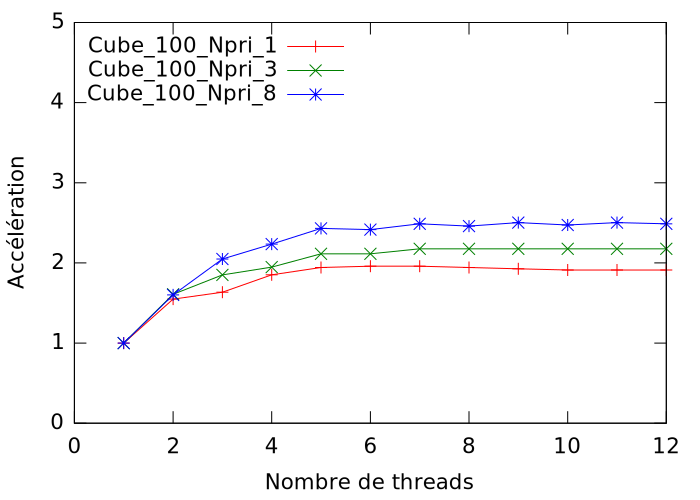
\includegraphics[width=0.7\textwidth]{res_spmv_omp}
  \caption{Accélération du produit matrice vecteur creux sur Rostand en mémoire partagée.}
  \label{fig:res_spmv_omp_rostand}
\end{figure}

%   (-_-)   %
\begin{figure}[t!]
  \centering
  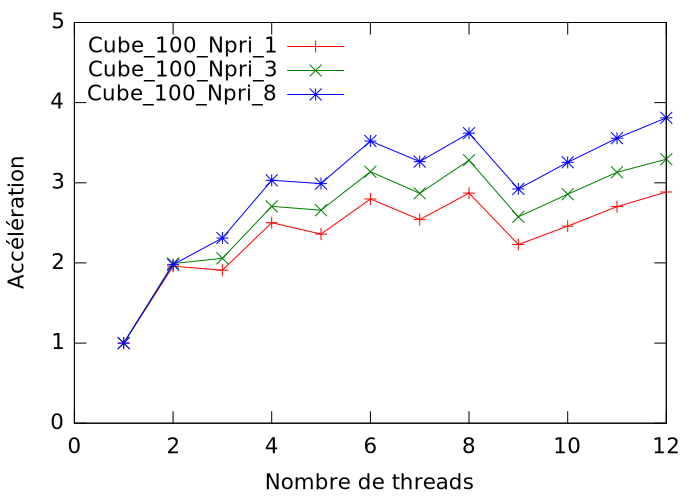
\includegraphics[width=0.7\textwidth]{res_spmv_mpi}
  \caption{Accélération du produit matrice vecteur creux sur Rostand en mémoire distribuée.}
  \label{fig:res_spmv_mpi_rostand}
\end{figure}
